\documentclass{article}

\usepackage{graphicx}
\usepackage{hyperref}
\usepackage{bm}
\usepackage{float}
\restylefloat{table}

\usepackage{listings}
\usepackage{color}
\usepackage{amsmath}

\DeclareUnicodeCharacter{2212}{-}

\usepackage[margin=1.25in]{geometry}

\definecolor{dkgreen}{rgb}{0,0.6,0}
\definecolor{gray}{rgb}{0.5,0.5,0.5}
\definecolor{mauve}{rgb}{0.86,0.27,0.22}
\DeclareRobustCommand\iff{\;\Longleftrightarrow\;}

\lstset{frame=tb,
  language=python,
  aboveskip=3mm,
  belowskip=3mm,
  showstringspaces=false,
  columns=flexible,
  basicstyle={\small\ttfamily},
  numbers=left,
  stepnumber=1,
  numberstyle=\tiny\color{gray},
  keywordstyle=\color{blue},
  commentstyle=\color{dkgreen},
  stringstyle=\color{mauve},
  breaklines=true,
  breakatwhitespace=true,
  tabsize=3
}

\title{CS5200: Final Exam} % Title of the assignment

\author{Matthew Whitesides\\ \texttt{mbwxd4@umsystem.edu}} % Author name and email address

\date{\today} % University, school and/or department name(s) and a date

%----------------------------------------------------------------------------------------

\begin{document}

  \maketitle % Print the title

  \textit{I, Matthew Whitesides, certify that all the material in this PDF file is my original work, that I did not discuss these questions with anyone other than my instructor, and that I did not copy work from anyone for this examination.}
 
  \begin{enumerate}
    \item \textbf{Hamiltonian Paths and Cycles}.
    
    Please refer to the following labeled nodes version of the graph for some of the questions.\\
    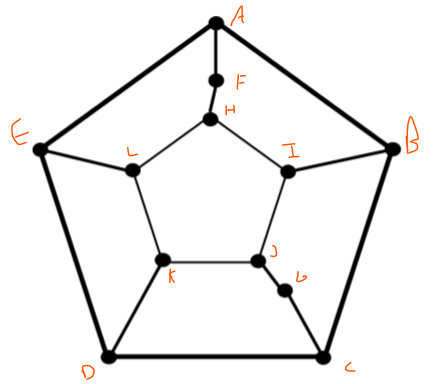
\includegraphics[scale=0.75]{1_Graph.png}

    \begin{enumerate}
        \item A Hamiltonian Path is defined as, "a graph path between two vertices of a graph that visits each vertex exactly once". Which yes this graph does have at least one. 
        
        For example the path in the labeled version above: 
        
        ${A \rightarrow F \rightarrow H \rightarrow I \rightarrow B \rightarrow C \rightarrow G \rightarrow J \rightarrow K \rightarrow D \rightarrow L}$ 
        
        would be a Hamiltonian Path.

        \item A Hamiltonian Cycle is defined as, " is a graph cycle (i.e., closed-loop) through a graph that visits each node exactly once.".
 
        Given a node has to be used once, each node that has a degree of 2 would have to have both of its edges used therefore edges (A,F),(F, H) and (J, G)(G, C) must be part of our cycle if one exists. 
        
        However, if we must include these four edges note that no matter which direction we attempt to get to vertices (A, H) and (J, G) we form a closed sub-circuit. 
        See the graph below to demonstrate this note the blue are edges we know must be in there and red and orange are two possible paths to those edges and both form a closed-loop without including all the other vertices.

        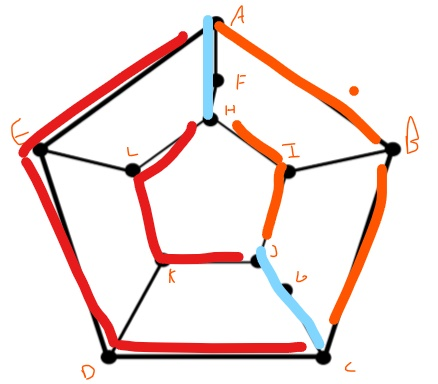
\includegraphics[scale=0.3]{1_Graph2.jpg}

        Therefore we know that this graph has no Hamiltonian cycle.

        \item
        \begin{itemize}          
          \item \textbf{The Problem.}
          \begin{itemize}
            \item We want to prove an n-dimensional cube contains a Hamiltonian Cycle. 
            \item An n-dimensional cube is defined as follows. It consists of the 2n vertices of the form $(a_0, a_1, ..., a_n)$ where each $a_i$ is either 0 or 1.
            \item Hamiltonian Cycle is defined as, " is a graph cycle (i.e., closed loop) through a graph that visits each node exactly once.".
            \item Our domain of n is any positive natural number in $n \ge 2$. As 0 would mean no edges or vertices and would be nothing, 1 would just be a line of two vertices which would not contain any cycles therefore not Hamiltonian, and a negative numbers of edges does not make sense.
          \end{itemize}
          \item \textbf{Check the base case plus one.}
          \begin{itemize}
            \item Base case: $n = 2$: This is true as this is just a square with 4 vertices and 4 edges, and if you simply use every edge you have formed a Hamiltonian cycle.
            
            I.e. if you go though $(0,0) \rightarrow (0,1) \rightarrow (1,1) \rightarrow (1,0) \rightarrow returns\;to\;(0,0)$.
            \item $n = 3$: This would form a cube which we could represent with the following graph (if you convert the letters to A = (0,0,0), B = (0,0,1).. etc:             
            
            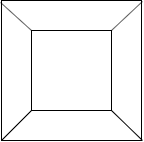
\includegraphics[scale=0.5]{cube.png}

            Which we can see has a Hamiltonian cycle if you follow the path:
            
            ${000 \rightarrow 001 \rightarrow 011 \rightarrow 010 \rightarrow 110 \rightarrow 111 \rightarrow 101 \rightarrow 100 \rightarrow 000}$.
          \end{itemize}
          \item \textbf{The Inductive Hypothesis.}
          \begin{itemize}
            \item Lets assume using the induction Hypothesis that an (n - 1) dimensional cube does in fact contain a Hamiltonian Cycle.
            \item We can agree that cube n is essentially cube (n - 1) with all adjacent edges connected to another (n - 1) cube.
            \item Lets define our n-dimensional cube as $C^n$.
            \item Therefore say for each vertex $v \in C^{n - 1}$ there is an adjacent vertex $v \in C'^{n - 1}$ that forms $C^n$.
            \item We can show this by our base cases of $n = 2$ is $(00, 01, 10, 11)$ then $n = 3$ is $(000, 001, 010, 011, 100, 101, 110, 111)$ .
            \item So we know that an n-cube contains $2^{n−1}n$ edges and $2^(n - 1) * 2$ vertices therefore we have an extra $2^{(-1 + n)} (-2 + n)$ edges connecting two adjacent $(n - 1)$ cubes. 
            \item We can also represent cube $n - 1$ within cube $n$ but adding a 0 in front of cube n's vertices (i.e. n = 2 is contained in (000, 001, 010, 011)) which we can call $v \in (0,1)^{n-1}$.
            \item And we can form a path from every edge $0_{v \in cube(n - 1)}$ like shown in the example above, except for the edge that goes though $0_n$ (or all zeros). This leaves an edge to connect to vertex $1_{v \in cube(n - 1)}$, then a path back to $0_n$.
            \item I.e. in the simple case n = 1 to n = 2. We have $v \in (0, 1)^1$ takes $0_{v \in cube(2 - 1)}$ or $00, 01$ connects those, then connects to $1_{v \in cube(2 - 1)}$ is $10, 11$ and finally back to $00$ to form the cycle.
            \item This using the Inductive Hypothesis can be scaled up to any $n \geq 2$. 
        \end{itemize}
        \item \textbf{Conclusion.}        
        Therefore we have proven using the inductive Hypothesis that any n-dimensional cube where $n \ge 2$ does contain a Hamiltonian Cycle.
      \end{itemize}
    \end{enumerate}

    \item \textbf{General Graph Theory}.
    \begin{enumerate}
        \item \textbf{(Max Flow / Min Cut):}
        
        The minimal cut of the given transport network are simply the cut through the output of the input node S or the input to the sink node that cuts through edges $\{(g,a), (g, f), (g, s)\}$ or $\{(d,t), (g,t), (j,t)\}$. 
        As shown below:

        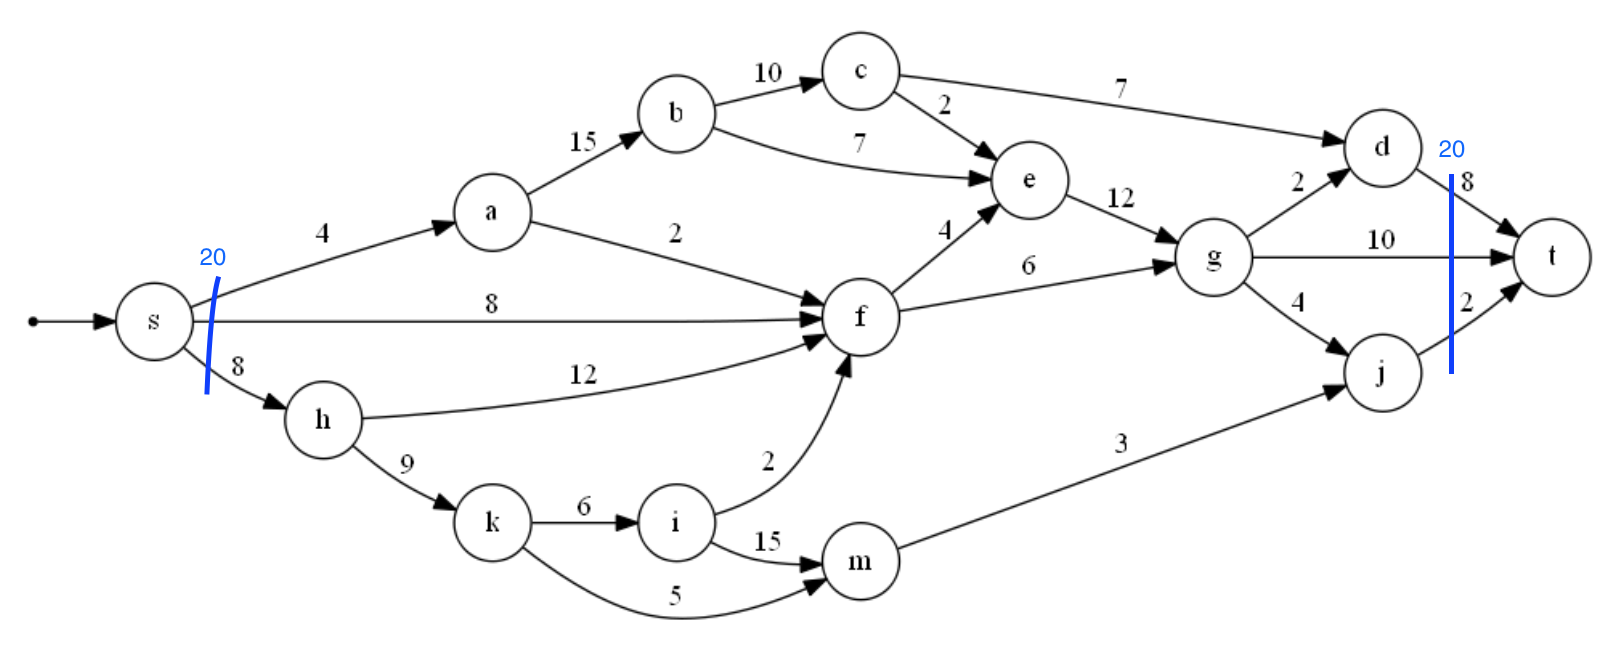
\includegraphics[scale=0.4]{2a}

        Therefore due the Max Flow / Min Cut theorem the maximal flow of the network is \bm{$f = 20$}.

        \item \textbf{(Handshaking):}
        
        Let's try a bit of a backward induction approach.
        
        If there are $N = 2$ people at the party then each person would have shaken hands with $(N - 1)$ person, e.g. the person other than John shook hands with one person which must be John. \\

        So if $Q(n)$ is the problem in question given $n = 2$ people how many hands did John shake then $Q(2) = 1$. \\

        Now if $N = 3$ than we have John and two others which at most could have shaken hands with $(N - 1)$ person so the other handshakes would be $(N - 1), (N - 2)$ or $(2),(1)$.         
        Therefore the Person with two handshakes would have shook John and Person 2, then Person 2 would have just shook hands with Person 1 so John would have 1 handshake. \\

        If $N = 4$ we have a graph like $V = \{A, B, C, John\}$ then if F is a function of handshakes 
        
        $F(A) = (N - 1) = \{B, C, John\}$
        
        $F(B) = (N - 2)\;People = \{A, John\}$
        
        $F(C) = (N - 3)\;People = \{A\}$ 
        
        therefore $F(John) = ? = \{A, B\}$ or 2 handshakes. \\

        If we scale this up we can deduce John will shake hands with $N//2$ people or if there are 10 people at the part John will shake hands with \textbf{5 people}.
        \item \textbf{(Vertex Degrees):}
        
        We want to prove every graph with $n \geq 2$ nodes must have at least two vertices having the same degree. \\
                
        First lets start with the possible degrees any given vertex can have in the graph with $n = num\;vertices$, then the range of possible degrees a vertex can have is $[1, n - 1]$. \\
        
        Therefore since the number of available options for $n$ vertices is $n - 1$ in the worst case we have at least one vertex that would have to share a degree with another one, since $n > (n - 1)$. \\
    
        Now if we take any graph that contains just a single pair of vertices we have a range of just $[1,1]$ possible degrees for each vertex. Therefore using the above proof the only degrees available to each vertex is a degree of 1. Just like a graph of $(A)-(B)$.

        \item \textbf{Connectedness:}
        
        To prove that $G'$ is connected when $G$ is disconnected let's start off saying that $G$ is disconnected. We just need to prove that $G'$ is connected.

        Lets say $(u, v) \notin G$ i.e. $(u, v)$ are a vertex edge pair that does not exist in graph $G$, that means by definition that $(u, v) \in G'$ or $(u, v)$ are in $G$.
       
        Now since $G$ is disconnected into multiple sub-graphs any edge $(u, v) \in G$ are part of a sub-graph, therefore any edge $(u', v')$ that would connect two vertices in disconnect sub-graphs must exist in $G'$.
       
        Finally, since $G$ is disconnected there is always an edge that does not exist from $v$ to any other $component\;subgraphs \in G$ meaning in the inverse $G'$ there must exist a vertex edge from each vertex in one sub-graph to the other component sub-graph(s).
       
        I.e. if you take two component sub-graphs edges $G = {(A)}, {(B,C)}$ must become $G' = {(A,B),(A,C)}$.

        \item \textbf{Chess:}
        
        First, let's establish the number of possible moves a Knight can have. When it's free in every direction it has 6 possible moves when it's is in it's starting position or up against one wall there are 3, possible moves, and when it's in a corner there are 2 possible moves.

        Therefore we can create and $8*8$ or $64$ node graph with each node having a degree equal to the valid possible moves for that node and connected to the nodes where the knight would end up if doing those moves. Once we have that graph we would look for a Eulerian path or a path that goes through each node exactly once.
       
        However even we know that by definition a Eulerian path "is necessary that zero or two vertices have an odd degree;", which our nodes that have a degree of 3 where the knights up against the walls are greater than 2 as there's 4 walls and multiple positions on the walls.
       
        Therefore we know we cannot form a path in our graph that hits each node exactly once and thus the knight cannot move and hit each move exactly once.

        \item \textbf{Two Coloring:}
        
        A graph is two colorable if it is a Bipartite graph and by definition of a Bipartite graph, "a bipartite graph is a graph that does not contain any odd-length cycles.". 

        Now unfortunately since we have an even number of vertices with an odd number of edges there must be at least one vertex that creates an odd length cycle. 
       
        Therefore we can not make a planar graph with 17 edges, and 10 vertices that can be 2-colored.
    \end{enumerate}

    \item \textbf{NP Complete Problems}.
    
    Note: Anytime I'm referencing the "book" I am referring to, "Introduction to Algorithms, 3rd Edition (The MIT Press) 3rd Edition by Thomas H. Cormen".
 
    \begin{enumerate}
      \item This particular problem is closely related to the "Circuit Satisfiability" problem in the book on p.1070 (see the book for full proof). Which is an \textbf{NP-Complete} problem on weather any given inputs in a circuit can produce a true output.
      You can pretty easily tell this problem in NP by simply taking a given solution and running it through the circuit to verify the faulty gate gives the same value no matter then input. 
      However, we know this type of problem is NP-Hard this proof essentially boils down to there's a polynomial-time number of input elements for every state in the circuit so even if a polynomial-time algorithm existed to verify one state each state would require a separate polynomial-time language. 
      
      \item I believe this problem is \textbf{NP-Complete}, if each node in a graph has a degree of two or less then it's essentially just a path with one in and one out edge for each node which is exactly what a "Hamiltonian Path" is, which is known to be NP-Complete, see book chapter 34.2 for proof.
      This problem is in NP as we can simply test in O(n) linear time if each node does have a degree of two or less. Also, this problem is closely related to the "Hamiltonian Cycle" problem which is NP-Complete which is just a Hamiltonian Path that ends at the same point it began. 
      Also, it's related to the "Circuit Satisfiability" problem we discussed in the previous question.
    
      \item We know that a minimum weight spanning tree (MST) can be found in \textbf{Polynomial Time} see book p.624 for an example of an O(E lg V) algorithm, and all we have to do once we have the MST is check if the total weight is less than some number K and you have your answer. 
      Therefore the problem is not NP-Hard and not NP-Complete. 
    
      \item Since we're not looking for the optimal scheduling solution we are just looking to see if we can schedule tasks under some constant time I call this solvable in \textbf{Polynomial Time} see book p.443 for an example of a task-scheduling solution. 
      Once we've found a minimum scheduling time we just need to check if it is under the given completion deadline. 
    
      \item First we can tell this problem is in NP easily by checking if our solution has each subset of vertices in $V_i \leq K$ and sum of weights of edges $V_i, V_j \leq J$ in at most $O(n^2)$ time. However, we are given Vertices, Edges, the sum of vertices, and the sum of edges.
      This is similar to the "Clique" problem, see book p.1087 with an added layer of complexity and that problem has been proven to be \textbf{NP-Complete}.      
    \end{enumerate}

    \item \textbf{Red-Black Trees, B-Trees, and Binary Search Trees}.
    
    \begin{enumerate}
      \item Below is an implementation of a Red-Black Tree based on the algorithm in the book on p.315. Code is also available in the zip file in a folder named 4 and a file named 4a.py.
      
      \begin{lstlisting}
class Node():
    """
    Class to contain a Red Black Tree Graph Bode properties.
    Specifically the key, p value, left, right and color. 
    """
    def __init__(self, key, left, right, color):
        self.key = key
        self.p = None
        self.left = left
        self.right = right
        self.color = color

class RBTree():
    """
    Class to contain a Red Black Tree Graph
    and preform insert and printing functionality.
    """
    def __init__(self):
        self.NIL = Node(0, None, None, "BLACK")
        self.root = self.NIL
        
    def print_tree(self):
        self.print_util(self.root, "", True)

    def print_util(self, node, tab, rightmost):
        if node != self.NIL:
            print(tab, end = "")            
            
            if rightmost:
                print("Right:", end = "")
            else:
                print("Left:", end = "")
            tab += "  "
                
            print("(" + str(node.key), node.color + ")")
            
            self.print_util(node.left, tab, False)
            self.print_util(node.right, tab, True)
    
    def get_height(self):
        return self.get_height_util(self.root, 0)
    
    def get_height_util(self, node, height):
        if node != self.NIL:
            height = self.get_height_util(node.right, height + 1)
        return height
        
    def rb_insert(self, z):
        """
        Inserts a new node with the value of z into this class instance's RB Tree.
        Uses the algorithm layed out in the book on p.315
        ----------
        Parameters
            z : int
                The value to insert into the tree.
        """
        z = Node(z, self.NIL, self.NIL, "RED")

        y = None
        x = self.root

        while x != self.NIL:
            y = x
            if z.key < x.key:
                x = x.left
            else:
                x = x.right

        z.p = y
        if y == None:
            self.root = z
        elif z.key < y.key:
            y.left = z
        else:
            y.right = z

        if z.p == None:
            z.color = "BLACK"
            return

        if z.p.p == None:
            return

        self.rb_insert_fixup(z)

    def rb_insert_fixup(self, z):
        """
        Preforms a "fixup" on the classes RBTree fixup implements the following logic.        
        If z is a root, color it black.
        If z's parent is red, then z's grandparent must be black.
        Let y be z's grandparent's other child.
        Fix depends on whether y is red or black.
        ----------
        Parameters
            z : Node
                The node to be "fixed".
        """
        while z.p.color == "RED":
            if z.p == z.p.p.right:
                u = z.p.p.left
                if u.color == "RED":
                    u.color = "BLACK"
                    z.p.color = "BLACK"
                    z.p.p.color = "RED"
                    z = z.p.p
                else:
                    if z == z.p.left:
                        z = z.p
                        self.right_rotate(z)

                    z.p.color = "BLACK"
                    z.p.p.color = "RED"
                    self.left_rotate(z.p.p)
            else:
                u = z.p.p.right

                if u.color == "RED":
                    u.color = "BLACK"
                    z.p.color = "BLACK"
                    z.p.p.color = "RED"
                    z = z.p.p
                else:
                    if z == z.p.right:
                        z = z.p
                        self.left_rotate(z)

                    z.p.color = "BLACK"
                    z.p.p.color = "RED"
                    self.right_rotate(z.p.p)

            if z == self.root:
                break

        self.root.color = "BLACK"

    def right_rotate(self, x):
        """
        Rotates the given node in a clockwise direction
        up the tree and adjests its siblings.
        ----------
        Parameters
            x : Node
                The node to be rotated.
        """        
        y = x.left
        x.left = y.right
        if y.right != self.NIL:
            y.right.p = x

        y.p = x.p
        if x.p == None:
            self.root = y
        elif x == x.p.right:
            x.p.right = y
        else:
            x.p.left = y

        y.right = x
        x.p = y

    def left_rotate(self, x):
        """
        Rotates the given node in a counter-clockwise direction
        down the tree and adjests its siblings.
        ----------
        Parameters
            x : Node
                The node to be rotated.
        """           
        y = x.right
        x.right = y.left
        if y.left != self.NIL:
            y.left.p = x

        y.p = x.p
        if x.p == None:
            self.root = y
        elif x == x.p.left:
            x.p.left = y
        else:
            x.p.right = y

        y.left = x
        x.p = y   
      \end{lstlisting}

      Test output based on the graph shown in the book p. 314 figure 13.3.

      \begin{lstlisting}
tree = RBTree()
tree.rb_insert(7)
tree.rb_insert(4)
tree.rb_insert(11)
tree.rb_insert(3)
tree.rb_insert(6)
tree.rb_insert(9)
tree.rb_insert(18)
tree.rb_insert(2)
tree.rb_insert(14)
tree.rb_insert(19)
tree.rb_insert(12)
tree.rb_insert(17)
tree.rb_insert(22)
tree.rb_insert(20)

print("RBTree Height:", tree.get_height())
tree.print_tree()       

# Output:
# RBTree Height: 5
# Right:(7 BLACK)
#   Left:(4 BLACK)
#     Left:(3 BLACK)
#       Left:(2 RED)
#     Right:(6 BLACK)
#   Right:(11 BLACK)
#     Left:(9 BLACK)
#     Right:(18 RED)
#       Left:(14 BLACK)
#         Left:(12 RED)
#         Right:(17 RED)
#       Right:(20 BLACK)
#         Left:(19 RED)
#         Right:(22 RED)
      \end{lstlisting}


      \item Below is the code used to generate 10 files of 10,000 random integers. See Zip file in folder 4 for all data files and 4b.py for full implementation and code of the analysis below.
      
      \begin{lstlisting}
import random
import time
import statistics

for i in range(10):
    file_name = "Data{0}.txt".format(str(i))
    rn = [random.randint(1,10000) for i in range(10000)]
    f = open(file_name, "w+")
    for r in rn: 
        f.write(str(r) + "\n")

f.close()

for i in range(10):
  file_name = "Data{0}.txt".format(str(i))
  with open(file_name) as f:
      data_str = f.readlines()
  data.append([int(x.strip()) for x in data_str])

print(len(data))

# Output:
# 10
      \end{lstlisting}

      Below is the analysis of the RB Tree algorithm implemented above, see 4b.py for full code. 

      \begin{lstlisting}
heights = []
times = []

for i in range(10):
    start = time.time()
    
    tree = RBTree()
    for value in data[i]:
        tree.rb_insert(value)
    
    end = time.time()
    
    heights.append(tree.get_height())
    times.append(end - start)

    
print("RBTrees Heights:", str(heights))
print("RBTrees Times:", str(times))
print("")
print("RBTrees Heights Mean:", statistics.mean(heights))
print("RBTrees Heights median:", statistics.median(heights))
print("RBTrees Heights Standard Dev:", statistics.stdev(heights))
print("")
print("RBTrees Times Mean:", statistics.mean(times))
print("RBTrees Times median:", statistics.median(times))
print("RBTrees Times Standard Dev:", statistics.stdev(times))

# Output:
# RBTrees Heights: [14, 13, 14, 13, 15, 14, 14, 13, 15, 12]
# RBTrees Times: [0.07790899276733398, 0.1125800609588623, 0.07030510902404785, 0.06880617141723633, 0.06974482536315918, 0.06842374801635742, 0.12203192710876465, 0.06870102882385254, 0.06848478317260742, 0.0690760612487793]

# RBTrees Heights Mean: 13.7
# RBTrees Heights median: 14.0
# RBTrees Heights Standard Dev: 0.9486832980505138

# RBTrees Times Mean: 0.0796062707901001
# RBTrees Times median: 0.06941044330596924
# RBTrees Times Standard Dev: 0.02019085514989934
      \end{lstlisting}

      Next is my analysis of my BST algorithm from Prelim2, see 4b\_BST.py for full code.

    \begin{lstlisting}
class Node: 
    def __init__(self, v): 
        self.key = v 
        self.left = None
        self.right = None
                
def tree_insert(T, z): 
    y = None
    x = T
    while x:
        y = x
        if z.key < x.key:
            x = x.left
        else: x = x.right
    if y is None:
        T = z
    elif z.key < y.key:
        y.left = z
    else: y.right = z
                
def inorder_traversal(T): 
    if T: 
        inorder_traversal(T.left) 
        print(T.key, end=", ") 
        inorder_traversal(T.right)
        
def get_height(T):
    return get_height_util(T, 0)

def get_height_util(T, height):
    if T:
        height = get_height_util(T.left, height + 1)
    return height
    \end{lstlisting}

    BST analysis.

    \begin{lstlisting}
heights = []
times = []

for i in range(10):
    start = time.time()
    
    tree = Node(10000)
    for value in data[i]:
        tree_insert(tree, Node(value))
    
    end = time.time()
    
    heights.append(get_height(tree))
    times.append(end - start)

    
print("BST Heights:", str(heights))
print("BST Times:", str(times))
print("")
print("BST heights Mean:", statistics.mean(heights))
print("BST heights median:", statistics.median(heights))
print("BST heights Standard Dev:", statistics.stdev(heights))
print("")
print("BST Times Mean:", statistics.mean(times))
print("BST Times median:", statistics.median(times))
print("BST Times Standard Dev:", statistics.stdev(times))

# Output:
# BST Heights: [8, 10, 12, 14, 7, 10, 11, 10, 4, 12]
# BST Times: [0.04905128479003906, 0.04745912551879883, 0.04601430892944336, 0.06760406494140625, 0.04880189895629883, 0.04637598991394043, 0.04508614540100098, 0.04470682144165039, 0.07152700424194336, 0.048017024993896484]

# BST heights Mean: 9.8
# BST heights median: 10.0
# BST heights Standard Dev: 2.859681411936962

# BST Times Mean: 0.0514643669128418
# BST Times median: 0.047738075256347656
# BST Times Standard Dev: 0.009694087189213559
    \end{lstlisting}

    Finally is my analysis of my B-Tree algorithm from Prelim2, see 4b\_BTree.py for full code.

    \begin{lstlisting}
class Node(object):
    def __init__(self):
        self.leaf = False
        self.keys = []
        self.c    = []
        
    def print_node(self):
        if self.leaf:
            return "Leaf node:{}".format(self.keys)
        return "Node: {}\nChildren: {}\n".format(self.keys, [child.print_node() for child in self.c])

class BTree():
    def b_tree_create(self, t):
        x = Node()
        x.leaf = True
        self.t = t
        self.root = x
        
    def b_tree_split_child(self, x, i):
        z = Node()
        y = x.c[i]
        z.leaf = y.leaf
        t = self.t
        x.c.insert(i + 1, z)        
        x.keys.insert(i, y.keys[t - 1])  
        
        for j in range(t - 1):
            if len(z.keys) < t - 1:
                z.keys.append(0)
            z.keys[j] = y.keys[j  + t]
        y.keys = y.keys[0: (t - 1)]
        
        if not y.leaf:
            z.keys = y.keys[t: (2*t - 1)]
            y.keys = y.keys[0: (t-1)]

    def b_tree_insert(self, k):
        r = self.root
        if len(r.keys) == (2 * self.t) - 1:
            s = Node()
            self.root = s
            s.c.insert(0, r)
            self.b_tree_split_child(s, 0)  
            self.b_tree_insert_nonfull(s, k)
        else: self.b_tree_insert_nonfull(r, k)
    
    def b_tree_insert_nonfull(self, x, k):
        i = len(x.keys) - 1
        if x.leaf or len(x.c) is 0:
            x.keys.insert(len(x.keys), 0)
            while i >= 0 and k < x.keys[i]:
                x.keys[i + 1] = x.keys[i]
                i = i - 1
            x.keys[i + 1] = k
        else: 
            while i >= 0 and k < x.keys[i]:
                i = i - 1            
            i = i + 1
            if len(x.c[i].keys) == (2 * self.t) - 1:
                self.b_tree_split_child(x, i)
                if k > x.keys[i]:
                    i = i + 1
            self.b_tree_insert_nonfull(x.c[i], k) 
    
    def b_tree_delete(self, k):
        (n, i) = self.find(k)
        if n is None:
            return None
        
        if n.leaf:
            del n.keys[i]
        else:
            k = n.keys[i]
            if len(n.c[i]) >= self.t:
                pred = n.c[i]
                while not curr.leaf:
                    pred = curr.c[len(curr.c) - 1]
                n.keys[i] = pred
                b_tree_delete(pred)
                
            elif len(n.c[i + 1]) >= self.t:
                succ = n.c[i + 1]
                while not curr.leaf:
                    succ = succ.c[0]
                n.keys[i] = succ
                b_tree_delete(succ)
    
    def find(self, k, x = None):
        if isinstance(x, Node):
            i = 0            
            while i < len(x.keys) and k > x.keys[i]:
                i = i + 1
            if i < len(x.keys) and k == x.keys[i]: return (x, i)
            elif x.leaf: return (None, 0)
            else: return self.find(k, x.c[i])
        else: return self.find(k, self.root)
    
    def print_tree(self):
        out = self.root.print_node()
        out += '\n'.join([child.print_node() for child in self.root.c])
        return out
    
    def get_height(self):
        return self.get_height_util(0)

    def get_height_util(self, height):
        height += 1
        height = len([child.print_node() for child in self.root.c])
        return height      
    \end{lstlisting}

    Analysis for B-Tree's:

    \begin{lstlisting}
heights = []
times = []

for i in range(10):
    start = time.time()
    
    tree = BTree()
    tree.b_tree_create(1000)
    for value in data[i]:
        tree.b_tree_insert(value)
    
    end = time.time()
    
    heights.append(tree.get_height())
    times.append(end - start)

    
print("B-Tree Heights:", str(heights))
print("B-Tree Times:", str(times))
print("")
print("B-Tree heights Mean:", statistics.mean(heights))
print("B-Tree heights median:", statistics.median(heights))
print("B-Tree heights Standard Dev:", statistics.stdev(heights))
print("")
print("B-Tree Times Mean:", statistics.mean(times))
print("B-Tree Times median:", statistics.median(times))
print("B-Tree Times Standard Dev:", statistics.stdev(times))     

# Output:
# B-Tree Heights: [8, 8, 8, 8, 8, 8, 8, 8, 8, 8]
# B-Tree Times: [2.26718807220459, 2.235520839691162, 2.2249579429626465, 2.3519208431243896, 2.4345662593841553, 2.302553176879883, 2.6907920837402344, 2.6656839847564697, 2.4060938358306885, 2.428806781768799]

# B-Tree heights Mean: 8
# B-Tree heights median: 8.0
# B-Tree heights Standard Dev: 0.0

# B-Tree Times Mean: 2.4008083820343016
# B-Tree Times median: 2.379007339477539
# B-Tree Times Standard Dev: 0.1647701717343564
    \end{lstlisting}

    Therefore our final analysis is the following. Interesting however B-Trees are heavily dependent on the initial level set for them to create off of this would probably need to be tweaked.

    \begin{lstlisting}      
RBTrees Heights Mean: 13.7
RBTrees Heights median: 14.0
RBTrees Heights Standard Dev: 0.9486832980505138

RBTrees Times Mean: 0.0796062707901001
RBTrees Times median: 0.06941044330596924
RBTrees Times Standard Dev: 0.02019085514989934

BST heights Mean: 9.8
BST heights median: 10.0
BST heights Standard Dev: 2.859681411936962

BST Times Mean: 0.0514643669128418
BST Times median: 0.047738075256347656
BST Times Standard Dev: 0.009694087189213559

B-Tree heights Mean: 8
B-Tree heights median: 8.0
B-Tree heights Standard Dev: 0.0

B-Tree Times Mean: 2.4008083820343016
B-Tree Times median: 2.379007339477539
B-Tree Times Standard Dev: 0.1647701717343564      
    \end{lstlisting}

    \end{enumerate}

    \item \textbf{More Graph Algorithms}.
    
    A bit of setup first we'll see if I did this correctly, I'll explain the code that I used to breakup the GraphData.txt into a Forest of connected graphs. Then get into the individual questions asked. 

    Below is the code used to break up the GraphData.txt into a "Forest" of graphs, it reads in the GraphData.txt into an array of tuples, then using the Forest class it generates a list of connected component subgraphs in the graph.
    Then builds those into adjacent list graphs which will be used for the following questions.

    First the reading in the GraphData.txt code.

    \begin{lstlisting}
import sys

txt_data = [line.rstrip('\n').rstrip(')').lstrip('(') for line in open('GraphData.txt')]
graph_data = []

# Put graph data into a array of tuples.
for line in txt_data:
    split = line.split(',')
    if len(split) == 2:
        x = int(split[0])
        y = int(split[1])
        graph_data.append((x, y, abs(x - y)))
        
print(graph_data)        
    \end{lstlisting}

    Next is the Forest generation code.

    \begin{lstlisting}
class Forest():
    """
    Class to take in an unconnected list of tuples containing (vert1, vert2, weight) data.
    Split it into individual connected components.
    Convert the node labels into integers (0 ... n).
    Create an adjacency list for graph.
    Do the same for each found subgraph in the data.
    """
    def __init__(self, graph_data):
        """
        Initializes a new instance of the Forest class
        ----------
        Parameters
            graph_data : [(int, int, int)]
                The graph data to build the dict off of.
        """          
        self.graph_data = graph_data

        dicts = self.build_graph_dict(self.graph_data)        
        self.graph_dict = dicts[0]
        self.graph_dict_rev = dicts[1]                
        
        self.V = len(self.graph_dict)
        
        self.graph = self.build_adj_list(self.graph_data, self.graph_dict, self.V)
        self.cc = self.get_connected_components()
        
        self.forest_dicts = []
        self.forest = []
        self.forest_data = []
        self.build_connected_forest()

        print("Forest Info:")
        print("\tNumber of vertices:", str(self.V))
        print("\tNumber of edges:", len(self.graph_data))
        print("\tNumber of connected components in forest:", len(self.cc))
        
        for i in range(len(self.forest)):
            print("\t\tSubgraph {0}: ".format(i))
            print("\t\t\t# vertices:", len(self.forest_dicts[i][0]))            
            print("\t\t\t# edges:", len(self.forest_data[i]))            
        
    def build_graph_dict(self, graph_data):
        """
        Builds a dictionary containing the labels in the graph.
        ----------
        Parameters
            graph_data : [(int, int, int)]
                The graph data to build the dict off of.
        """        
        graph_dict = {}
        graph_dict_rev = {}
        i = 0

        for x in graph_data:
            if x[0] not in graph_dict:
                graph_dict[x[0]] = i
                graph_dict_rev[i] = x[0]
                i += 1
            if x[1] not in graph_dict:
                graph_dict[x[1]] = i
                graph_dict_rev[i] = x[1]
                i += 1

        return (graph_dict, graph_dict_rev)
        
    def build_adj_list(self, graph_data, graph_dict, length):
        """
        Builds an adjacency list of the given graph data.
        ----------
        Parameters
            graph_data : [(int, int, int)]
                The graph data to build the adj list off of.
            graph_dict : {}
                The graph data's dict.
            length : int
                The number of nodes in the graph.
        """          
        graph = [[(0, 0) for i in range(length)] for j in range(length)]

        for d in graph_data:
            x = graph_dict[d[0]]
            y = graph_dict[d[1]]
            graph[x][y] = (y, d[2])
            graph[y][x] = (x, d[2])
        
        return graph
            
    def build_connected_forest(self):
        """
        Builds an array of graphs from the separate components
        in the class's total graph data.
        """                  
        for c in self.cc:
            graph_data = []
            for x in c:
                for edge in self.find_edges(x):
                    if not self.edge_in_edges(edge, graph_data):
                        graph_data.append(edge)   

            d = self.build_graph_dict(graph_data)
            adj = self.build_adj_list(graph_data, d[0], len(d[0]))
            
            self.forest_dicts.append(d)
            self.forest_data.append(graph_data)
            self.forest.append(adj)
                
    def find_edges(self, v):
        """
        Gets the edges matching the given vertex from the graph data.
        ----------
        Parameters
            v : int
                The requested vertex.
        """                  
        edges = []
        for edge in self.graph_data:
            if edge[0] == self.graph_dict_rev[v] or edge[1] == self.graph_dict_rev[v]:
                edges.append(edge)

        return edges
    
    def edge_in_edges(self, edge, edges):
        """
        Checks if an edge already exists in the edges list.
        ----------
        Parameters
            edge : (int, int)
                The requested edge.
            edge : [(int, int)]
                The list of edges.
        """          
        for e in edges:
            if edge[0] == e[0] and edge[1] == e[1]:
                return True

        return False
            
    def print_cc_list(self):
        """
        Prints out the separate components from the forest.
        """          
        i = 0
        for cc in self.forest_data:
            print("\nComponent {0}:".format(str(i)))
            i += 1
            for c in cc:
                s = "["
                for x in c:
                    s += str(x) + ','
                s = s[:-1]
                s += "]"
                print(s)        
                
    def get_connected_components(self): 
        """
        Uses DFS to find connected components in the total graph.
        """           
        cc = [] 
        repeat = [] 
        
        for i in range(self.V): 
            repeat.append(False) 

        for v in range(self.V): 
            if not repeat[v]: 
                t = [] 
                cc.append(self.dfs(t, v, repeat)) 
        
        return cc 
    
    def dfs(self, t, v, repeat):
        """
        Uses the DFS algorithm to recursively scan through the graph looking for connected edges.
        ----------
        Parameters
            t : []
                The temp list used for checking existing values.
            v : int
                The new vertex to add.
            repeat : []
                The list of vertices that already exist in the component.
        """         
        repeat[v] = True
        t.append(v) 

        for i in self.graph[v]: 
            if not repeat[i[0]]: 
                t = self.dfs(t, i[0], repeat) 

        return t       
    \end{lstlisting}

    Then we can see the output of the forest for the GraphData.txt file.

    \begin{lstlisting}
forest = Forest(graph_data) 

# Output:
Forest Info:
	Number of vertices: 1426
	Number of edges: 2342
	Number of connected components in forest: 10
		Subgraph 0: 
			# vertices: 159
			# edges: 267
		Subgraph 1: 
			# vertices: 125
			# edges: 199
		Subgraph 2: 
			# vertices: 161
			# edges: 271
		Subgraph 3: 
			# vertices: 158
			# edges: 265
		Subgraph 4: 
			# vertices: 125
			# edges: 199
		Subgraph 5: 
			# vertices: 125
			# edges: 199
		Subgraph 6: 
			# vertices: 162
			# edges: 273
		Subgraph 7: 
			# vertices: 125
			# edges: 199
		Subgraph 8: 
			# vertices: 161
			# edges: 271
		Subgraph 9: 
			# vertices: 125
			# edges: 199        
    \end{lstlisting}

    Alright now onto the actual questions.

    \begin{enumerate}
        \item Below is my MST-Prim implementation used to find the Minimum Weight Spanning Tree from the trees in the GraphData.txt. See "5\textbackslash5a.py" and "5\textbackslash5a\_Output.txt" for the full implementation and output.
        
        \begin{lstlisting}
class Graph():
    """
    Class to contain the algorithms for MST-Prim and graph data.
    Graph data should be stored a an adjacency list with the matching nodes containing the weight of the edge.
    """
    def __init__(self, vertices, graph_dict):
        """
        Initializes a new instance of the Graph class
        ----------
        Parameters
            graph_dict : {}
                The graph dictionary containing the node labels.
        """        
        self.V = vertices 
        self.graph = [[0 for column in range(vertices)] for row in range(vertices)] 
        self.graph_dict = graph_dict
        
    def print_tree(self, p):
        """
        Prints out the MST tree and the total weight of the tree.
        ----------
        Parameters
            p : []
                The parent node.
        """             
        print("(Edge) - Weight")
        weight = 0
        
        for i in range(1, self.V): 
            print("(" + str(self.graph_dict[p[i]]) + ",", 
                    str(self.graph_dict[i]) + ")", 
                    "-", self.graph[i][p[i]][1])
            weight += int(self.graph[i][p[i]][1])
        
        print("Total weight:", weight)

    def extract_min(self, w, r):
        """
        Gets the minimum weight node of the vertices.
        ----------
        Parameters
            w : []
                The the weights to compare to.
            r : []
                The list of used nodes.
        """           
        min = sys.maxsize 

        for v in range(self.V): 
            if w[v] < min and not r[v]: 
                min = w[v] 
                i = v 

        return i 

    def mst_prim(self):
        """
        The MST-Prim algorithm implementation based off the book p. 634.
        """            
        w = [sys.maxsize] * self.V 
        p = [None] * self.V

        w[0] = 0 
        p[0] = -1
        r = [False] * self.V 

        for x in range(self.V): 
            u = self.extract_min(w, r) 
            r[u] = True
            for v in range(self.V): 
                if self.graph[u][v][1] > 0 and not r[v] and w[v] > self.graph[u][v][1]: 
                        w[v] = self.graph[u][v][1] 
                        p[v] = u 

        self.print_tree(p) 
        \end{lstlisting}

        Code used to generate the output and find the min tree.

        \begin{lstlisting}
for i in range(len(forest.forest)):
    print("Prim MST on Subgraph {0}:".format(i))
    verticies = len(forest.forest_dicts[i][0])
    data = forest.forest[i]
    graph_dict = forest.forest_dicts[i][1]
    g = Graph(verticies, graph_dict)
    g.graph = data
    g.mst_prim()
    print("")            

# Output:
Prim MST on Subgraph 0:
(Edge) - Weight
(277, 325) - 48
... See "5a\_Output.txt" in Zip file for full output.
        \end{lstlisting}        

        So finally we can see that the \textbf{MST of the sub-trees is 7540} in the subgraph component index 1. See "5\textbackslash5a\_Output.txt" for the edge list and the total weights and edges of the rest of the graph.

        \item Next is my implementation the find the shortest path of the trees using the Dijkstra Shortest-Paths algorithm from p.658 of the book. 
        Setup is the same as the intro Forest code, the new Graph class implements the algorithm.
        See "5\textbackslash5b.py" and "5\textbackslash5b\_Output.txt" for the full implementation and output.
        
        \begin{lstlisting}
import sys 

class Graph():   
    """
    Class to contain the algorithms for MST-Prim and graph data.
    Graph data should be stored a an adjacency list with the matching nodes containing the weight of the edge.
    """
    def __init__(self, vertices, graph_dict):
        """
        Initializes a new instance of the Graph class
        ----------
        Parameters
            graph_dict : {}
                The graph dictionary containing the node labels.
        """        
        self.V = vertices 
        self.graph = [[0 for column in range(vertices)] for row in range(vertices)] 
        self.graph_dict = graph_dict

    def print_all_pairs_shortest_path(self, s, i): 
        """
        Prints out the path length for each node in the graph.
        ----------
        Parameters
            s : int
                The starting node.
            i : []
                The starting node paths.
        """     
        print("(v1 -> v2) - Weighted Distance")
        max_weight = 0
        max_str = ""
        for node in range(self.V): 
            out = "({0} -> {1}) - {2}".format(self.graph_dict[s], self.graph_dict[node], i[node])
            print(out)
            if i[node] > max_weight:
                max_weight = i[node]
                max_str = out
        print("Max Path:", max_str)

    def extract_min(self, w, S): 
        """
        Gets the minimum weighted node from the start to each of the graph vertices.
        ----------
        Parameters
            w : int
                The starting node weights.
            S : []
                The set of node paths.
        """     
        min = sys.maxsize 

        for v in range(self.V): 
            if w[v] < min and S[v] == False: 
                min = w[v] 
                min_index = v 

        return min_index 

    def dijkstra(self, s): 
        """
        Preforms the Disjkstra Shortest Paths algorithm from the book p.658 (... and Wikipedia)
        ----------
        Parameters
            w : int
                The shortest path weight.
            s : []
                The source node.
        """           
        # Essentially INITIALIZE-SINGLE-SOURCE
        w = [sys.maxsize] * self.V 
        S = [False] * self.V 
        w[s] = 0

        for i in range(self.V): 
            u = self.extract_min(w, S) 
            S[u] = True

            # For each Vertex in Adj Graph
            for v in range(self.V): 
                if self.graph[u][v][1] > 0 and not S[v]:
                    if w[v] > w[u] + self.graph[u][v][1]: 
                        w[v] = w[u] + self.graph[u][v][1] 

        self.print_all_pairs_shortest_path(s, w)             
        \end{lstlisting}

        Next the code to generate the output:

        \begin{lstlisting}
forest = Forest(graph_data)
print("")
print("Dijkstra Shortest-Paths on Subgraph:", "1")
verticies = len(forest.forest_dicts[1][0])

for v in range(verticies):
    print("Path starting at vertex:", forest.forest_dicts[1][1][v])
    data = forest.forest[1]
    graph_dict = forest.forest_dicts[1][1]
    g = Graph(verticies, graph_dict)
    g.graph = data
    g.dijkstra(v)
    print("")            
    
# Output:
# Dijkstra Shortest-Paths on Subgraph: 1
# Path starting at vertex: 6499
# (v1 -> v2) - Weighted Distance
# (6499 -> 6499) - 0
# ... See "5b\_Output.txt" in Zip file for full output.
        \end{lstlisting}

        Now using this code we can look through the generated path weights and see that \textbf{The maximum of the shortest paths of the subtree found in part 1 (Subtree 1 in the output) is Vertex 6328 to 6313 with a path weight of 837}.
        And obviously the other path that also has this max weight is 6313 to 6328 with the same weight of 837.

        See "5\textbackslash5b\_Output.txt" in the zip file for the full path weight calculation for every node to every other node.

        \item Finally for finding the longest paths we can actually just modify our Depth First Search method we used to generate the adjacency lists. 
        Below is the code used to do the DFS and then to analyze every possible path from every node to each other node and build a max list of paths.
        obviously I would need to optimize a lof of the checking code is in lists because of the tuples i made out of the verticies but the DFS itself seems sound enough.
        As per usual see "5\textbackslash5c.py" and "5\textbackslash5c\_Output.txt" for full output and code.

        \begin{lstlisting}
class Graph():
    """
    Class to contain the algorithms for MST-Prim and graph data.
    Graph data should be stored a an adjacency list with the matching nodes containing the weight of the edge.
    """
    def __init__(self, vertices, graph_dict):
        """
        Initializes a new instance of the Graph class
        ----------
        Parameters
            graph_dict : {}
                The graph dictionary containing the node labels.
        """        
        self.V = vertices 
        self.graph = [[0 for column in range(vertices)] for row in range(vertices)] 
        self.graph_dict = graph_dict        
        
    def dfs(self, v, repeat = None, path = None):
        """
        Uses the DFS algorithm to recursively scan through the graph looking for 
        the longest path possible.
        ----------
        Parameters
            t : []
                The temp list used for checking existing values.
            v : int
                The new vertex to add.
            repeat : []
                The list of vertices that already exist in the component.
        """         
        if repeat is None: 
            repeat = []
        if path is None: 
            path = [v]

        repeat.append(v)

        paths = []
        for t in self.graph[v[0]]: 
            if not self.in_vertex_list(t, repeat): 
                new_path = path + [t]
                paths.append(tuple(new_path))
                paths.extend(self.dfs(t, repeat[:], new_path)) 

        return paths
    
    def in_vertex_list(self, v, verticies):
        """
        Helper method to check if a tuple vert is in a list of tuples
        ----------
        Parameters
            v : (,)
                The vert in question.
            verticies: []
                The list of verticies to check aginst.
        """  
        t = [vert for vert in verticies if vert[0] == v[0]]
        return len(t) > 0            
        \end{lstlisting}

        Code to analyze the graph data.

        \begin{lstlisting}
forest = Forest(graph_data) 
max_paths = []
max_length = 0

def in_path_list(path, paths):
    if len(paths) is 0:
        return False
    for p in paths:
        if len(p) is not len(path):
            continue
        if in_tup(p, path):
            return True
    return False

def in_tup(p, path):
    for i in range(len(p)):
        if p[i][0] is not path[i][0]:
            return False
    return True

for i in range(len(forest.forest)):
    verticies = len(forest.forest_dicts[i][0])
    data = forest.forest[i]
    graph_dict = forest.forest_dicts[i][1]
    g = Graph(verticies, graph_dict)
    g.graph = data
    
    # Find max possible paths.
    for vertex in graph_dict:
        paths = g.dfs((vertex, 0))
        for p in paths:
            length = len(p)
            if length >= max_length:
                if length > max_length:
                    max_paths = []
                    max_length = length                
                if not in_path_list(p, max_paths):
                    max_paths.append(p)
                    
print("\nMax paths that exist in GraphData.txt have a length of {}.".format(len(max_paths[0])))
# Print Possible Paths
for p in max_paths:
    s = ""
    for t in p:            
        s += str(graph_dict[t[0]]) + " -> "
    s = s[:-3]
    print(s)            
        \end{lstlisting}

        So using this code we have found the \textbf{maximum path length is 0, and 0 separate paths have that length}. Below are the actual paths of such length (See "5\textbackslash5a\_Output.txt" for full output).

    \end{enumerate}
    
    \item \textbf{GCD}.
    
    \begin{enumerate}
        \item If we know the two integers are even:
        
        \[GCD(p, p) = p\]
        
        Therefore:

        \[GCD(p, q) = p = 2 * (\frac{p}{2}) \iff p = q\]

        And we can say (where $d|a$ is the gcd(a, a)):

        \[d|p, d|q\;then\;\frac{d}{2}|\frac{p}{2}, \frac{d}{2}|\frac{q}{2}\]

        Since p and q are even we know $\frac{d}{2}$ is a common divisor of $\frac{p}{2}$ and $\frac{q}{2}$.

        And we know that 2 is a common divisor of $p$ and $q$.

        Thus we know that:

        \[GCD(\frac{p}{2},\frac{q}{2}) \geq \frac{d}{2}\]

        Since d is the gcd of (p, q), d/2 must be the maximum that the gcd of (p/2, q/2) could be, and obviously d = (d / 2) * 2. \\

        Also you could just say if (using theorem 31.3 from the book):

        \[GCD(p, q) = xp + yq\]
        \[xp + yq = 2(\frac{xp}{2} + \frac{yq}{2})\]

        \item In sort we want to prove the fact that because p is odd we know that 2 cannot be a common divisor of (p, q) so it wouldn't change anything to divide p by 1 or 2.\\
        
        If $p$ is odd and $q$ is even then obviously $p \neq q$,
        and we know that no odd number can be divided evenly by an even number so $GCD(p, q) \neq q$.\\

        Therefore $GCD(p, q) < q$, and since the $GCD(p, q) \neq 2$.\\

        So we have ruled out $q, 2$ as being possible divisors therefore using the above proof we can say $GCD(q, q/2) = q/2$.\\

        Also due to basic GCD rules we know $GCD(p, q) \leq p$ and $GCD(p, q) \leq q$ then we can say $GCD(p, q) = GCD(p, q/2)$ if $q$ is even and p is odd. 

        \item We know that an odd number minus an odd number gives an even number, therefore $p - q$ is even. That means (p - q) / 2 is a whole integer which is always true for GCD.\\
        
        And since $p > q$ $GCD(p, q) \neq p$.\\

        We also know from theorem 31.3 that $d | (a - b)$ implies that $GCD(p, q) = GCD(p - q, q)$ if $p - q > 0$ which in this case it is as $p > q$.\\

        And the last question we proved $GCD(p, q) = GCD(p, q / 2)$ if p is odd and q is even.\\

        Which we know $(p - q)$ is even and can just flip the properties around using theorem 31.6 ($GCD(a, b) = GCD(b, a)$).\\

        Which leaves us finally $GCD(p, q) = GCD((p - q) / 2, q)$.
        
        
        \item The following is an implementation based upon the previous three definitions and the EUCLID algorithm in the book chapter 31.2. Code also available in the zip file under 6.py.
        
        The main algorithm is in the gcd\_util() method as the main GCD converts the given number to a binary string and keeps itself separate from the recursion.
        
        \begin{lstlisting}
def gcd(p, q):
    """
    Formats the given numbers into binary and calculates the 
    greatest common divisor by calling the gcd_util method.
    ----------
    Parameters
        p : int
            The first number.
        q : int
            The second number.    
    -------
    Returns
        int
            The gcd in integer form.
    """
    p = format(p, 'b')
    q = format(q, 'b')
    result = gcd_util(p, q)
    return int(result, 2)

def gcd_util(p, q):
    """
    Calculates the greatest common divisor using recursive binary string manipulation.
    ----------
    Parameters
        p : int
            The first number.
        q : int
            The second number.      
    -------
    Returns
        int
            The gcd in binary string form.
    """
    # Base Cases
    if p == q:
        return p

    if is_zero(p):
        return p

    if is_zero(q):
        return q

    # Proof 6a: If p is even divide by two.
    if is_even(p):
        if is_even(q):
            return shift_left(gcd_util(shift_right(p), shift_right(q)))
        else:
            return gcd_util(shift_right(p), q)

    # Proof 6b: If p is odd and q is even.
    if (is_even(q)):
        return gcd_util(p, shift_right(q))

    # Proof 6c: If p and q are both odd and p > q.
    if is_greater(p, q):
        return gcd_util(shift_right(minus(p, q)), q)

    return gcd_util(shift_right(minus(q, p)), p)

def is_zero(s):
    return s == len(s) * '0'

def is_even(s):
    return s[len(s) - 1] == '0'

# Multiply by two, by adding a zero to the end.
def shift_left(s):
    return s + '0'

# Divide by two, by removing the last char.
def shift_right(s):
    return s[: -1]

def is_greater(x, y):
    if len(x) > len(y):
        return True
    return int(x, 2) > int(y, 2)

def minus(x, y):
    return format(int(x, 2) - int(y, 2), 'b')          
        \end{lstlisting}

        Next is some tests on 100 pairs of random numbers between 0 and 10,000,000, using the built in math.gcd function for validation that our our custom GCD algorithm works.

        \begin{lstlisting}
import math
import random

rand_nums = [(random.randrange(0, 10000000), random.randrange(0, 10000000)) for i in range(100)]

for n in rand_nums:
    my_gcd = gcd(n[0], n[1])
    math_gcd = math.gcd(n[0], n[1])
    valid = my_gcd == math_gcd
    s = "GCD({},{}) = {}: Valid = {}".format(str(n[0]), str(n[1]), str(my_gcd), str(valid))
    print(s)

# Output:
GCD(1538856,3119886) = 198: Valid = True
GCD(7914355,1511558) = 1: Valid = True
GCD(7689698,3196157) = 1: Valid = True
GCD(9215805,9153735) = 15: Valid = True
GCD(689520,6448224) = 48: Valid = True
GCD(1091935,8600069) = 1: Valid = True
GCD(6699525,3740816) = 1: Valid = True
GCD(8343132,1335031) = 1: Valid = True
GCD(5668326,6372101) = 1: Valid = True
GCD(507207,7191700) = 1: Valid = True
GCD(1657302,8695889) = 1: Valid = True
GCD(3895432,9300223) = 1: Valid = True
GCD(1447369,4070530) = 1: Valid = True
GCD(625554,7662878) = 2: Valid = True
GCD(4099520,9983340) = 20: Valid = True
GCD(4242430,8746934) = 2: Valid = True
GCD(4224013,9944584) = 1: Valid = True
GCD(7924562,8333583) = 1: Valid = True
GCD(3689938,7683761) = 1: Valid = True
GCD(2538929,5714762) = 1: Valid = True
GCD(7283602,6257603) = 1: Valid = True
GCD(6224831,3717497) = 1: Valid = True
GCD(9902804,5713719) = 1: Valid = True
GCD(3486538,444740) = 2: Valid = True
GCD(9727931,3666453) = 1: Valid = True
GCD(5103688,7288129) = 1: Valid = True
GCD(1813503,2072732) = 1: Valid = True
GCD(2335878,6392912) = 2: Valid = True
GCD(1346708,6402414) = 2: Valid = True
GCD(5094314,205662) = 2: Valid = True
GCD(6004650,5128461) = 3: Valid = True
GCD(9168461,9678714) = 1: Valid = True
GCD(2458709,4581295) = 1: Valid = True
GCD(8260594,8354852) = 2: Valid = True
GCD(8588868,6014742) = 6: Valid = True
GCD(9133893,3748095) = 9: Valid = True
GCD(2767474,8592140) = 2: Valid = True
GCD(2783352,1884924) = 12: Valid = True
GCD(1506689,8603835) = 1: Valid = True
GCD(972762,5818927) = 1: Valid = True
GCD(1469327,210559) = 1: Valid = True
GCD(4389611,5808938) = 1: Valid = True
GCD(4773064,9205376) = 8: Valid = True
GCD(9120320,5344503) = 1: Valid = True
GCD(3690248,7216206) = 2: Valid = True
GCD(5514667,1897652) = 1: Valid = True
GCD(9465515,520126) = 1: Valid = True
GCD(6947848,8186467) = 1: Valid = True
GCD(1520632,2273765) = 1: Valid = True
GCD(8056159,4056243) = 1: Valid = True
GCD(7370289,4497508) = 1: Valid = True
GCD(7926750,6743645) = 5: Valid = True
GCD(3834517,5254726) = 1: Valid = True
GCD(2354774,2429083) = 1: Valid = True
GCD(3100935,3779216) = 1: Valid = True
GCD(9000615,4923537) = 3: Valid = True
GCD(8504032,4515543) = 1: Valid = True
GCD(9668345,9586247) = 1: Valid = True
GCD(3410580,9316504) = 4: Valid = True
GCD(9976159,2307393) = 1: Valid = True
GCD(334049,561823) = 1: Valid = True
GCD(4302445,1028250) = 5: Valid = True
GCD(8887907,5956705) = 1: Valid = True
GCD(774851,7782759) = 29: Valid = True
GCD(143844,7501340) = 4: Valid = True
GCD(2954894,8403757) = 1: Valid = True
GCD(4775893,4355683) = 1: Valid = True
GCD(4349212,8702977) = 1: Valid = True
GCD(8748750,4768746) = 6: Valid = True
GCD(3654456,1339660) = 4: Valid = True
GCD(130625,4382430) = 5: Valid = True
GCD(7393393,8294257) = 1: Valid = True
GCD(74839,2065316) = 1: Valid = True
GCD(2836026,6028635) = 3: Valid = True
GCD(6656040,7303050) = 90: Valid = True
GCD(6582605,3174664) = 1: Valid = True
GCD(9037991,4158127) = 1: Valid = True
GCD(4374985,9406388) = 1: Valid = True
GCD(3431537,5710879) = 1: Valid = True
GCD(4522902,8356726) = 2: Valid = True
GCD(9645750,1487810) = 10: Valid = True
GCD(7797770,6749390) = 10: Valid = True
GCD(8849941,9409346) = 1: Valid = True
GCD(6701792,1346482) = 2: Valid = True
GCD(1297385,3483966) = 1: Valid = True
GCD(3011548,9145584) = 172: Valid = True
GCD(464411,8283354) = 1: Valid = True
GCD(2124342,4066508) = 2: Valid = True
GCD(3736756,8176411) = 1: Valid = True
GCD(34389,2818507) = 1: Valid = True
GCD(7083235,7095524) = 1: Valid = True
GCD(1535923,7422923) = 1: Valid = True
GCD(8946907,2019604) = 1: Valid = True
GCD(4951742,3698815) = 1: Valid = True
GCD(171714,7487361) = 3: Valid = True
GCD(9240535,5032304) = 1: Valid = True
GCD(6453503,5370161) = 1: Valid = True
GCD(9156934,2304982) = 2: Valid = True
GCD(9889135,3125602) = 1: Valid = True
GCD(9507098,4548646) = 2: Valid = True    
        \end{lstlisting}
    \end{enumerate}
  \end{enumerate}  % End of questions.
\end{document}
